\chapter{Finishing Decode}

\section{iDecode Module}
At this point, you have created all of the modules necessary to assemble the iDecode module.  Now you need to create a new module called iDecode.  The inputs and outputs can be determined by evaluating Figure~\ref{fig:decode_stage}.  Any signal that crosses the boundaries of the red box is an input or output.  Signals that do not cross the boundaries of the red box are signals that are internal to the iDecode module and should be declared internally in iDecode.  Please make sure to label signals consistently with lower case letters with words separated by underscores.  For example, read\_data1, write\_data, alu\_src.

\begin{figure}
	\caption{Expected Results}\label{fig:decode_stage}
	\begin{center}
		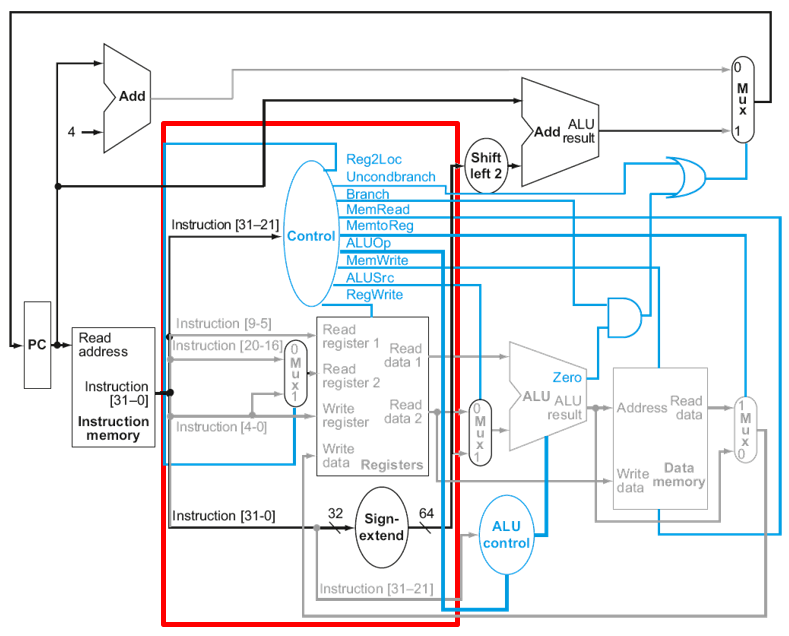
\includegraphics[width=4.75in]{../images/decode_stage.png}
	\end{center}
\end{figure} 


\section{iDecode Unit Test}
To verify that your iDecode module works correctly, you must first update your Expected Results Table. You should first add a row for every input and output of your iDecode module, then fill in all cells with expected values.  If a particular data item is not relevant for a particular instruction (for instance, sign\_extended\_output on an R-type instruction), then just put an X in that cell.  To ensure that we are testing each case, please update regData.data to reflect the following values:

\begin{enumerate}
	\item X19 = 10
	\item X20 = 30
	\item X21 = 0
	\item X22 = 16
\end{enumerate}

Now create a unit test for iDecode by providing the inputs for iDecode and verifying the outputs of iDecode.  For the instruction input, use the instructions from your Expected Results Table.  For arithmetic instructions, use the test bench to provide the correct value to the write\_data input, since we do not yet have an ALU to do the calculations.  Also, please use your test bench to provide a value of 20 to X9 in the first command (LDUR).

With your Expected Results Table in hand, you should be able to run the iDecode unit test and analyze your simulation outputs by going vertically down the simulation output, comparing the table to your simulation output.  While certain values will be offset in time, a single instruction should fall within a single clock cycle.  

\section{Integrating iFetch and iDecode}
Now that you have iDecode created and tested, you can test it with your iFetch module.  To do this, you need to create a file called datapath.v.  This will be your top-level file for your integrated datapath, analagous to the test bench files.  In this file, you should have an instance of iFetch and iDecode.  You should connect these two modules with wires by analyzing the full datapath diagram.  Since we do not have a full datapath yet, we need to have some "test bench" aspects to datapath.v.  Similarly to your iFetch test, you will want to create a reg for reset, pc\_src, and branch\_target.  Since we do not have all aspects of branching implemented, please keep pc\_src set to 0 for the duration of the test.  

Please update your instrData.data file to only contain the 10 instructions in your Expected Results Table.  The goal of datapath.v is to verify that the PC increments, each of these instructions is fetched at the appropriate time, and that the instruction executes properly.  You can verify the execution by comparing your results with your expected results table.     

\section{Your Assignment}

You are to:
\begin{enumerate}
\item Integrate all individual modules into the iDecode module.
\item Update your Expected Results Table to include all iDecode inputs and outputs.
\item Test the iDecode module with the instructions from the Expected Results Table.
\item Verify that your simulation results match your expected results.
\item Create datapath.v and integrate the iFetch and iDecode stages.
\item Verify that the results match the Expected Results Table.
\item Write a lab report according to the LabN format.  The focus of the report is the iDecode module, including testing it with iDecode\_test and integrating it with iFetch.  It does not need to describe the details of the submodules...you have already written a report on those.  Please consider datapath.v to be a testbench when writing the report.
\end{enumerate} 